% !TeX root = ../galois.tex

\chapter{Aplicaciones}

\section{Introducción. Radicales y resolubilidad.}

En este capítulo vamos a ver el \textit{Gran Torema de Galois}, que nos dice que un polinomio es \textit{resoluble por radicales} si y sólo si su grupo de Galois es \textit{resoluble}. Como es evidente, vamos a tener que introducir una serie de conceptos nuevos para desarrollar esta parte de la teoría.

\begin{dfn}[Radical]
    $R/K$ es \textbf{radical} si existe una cadena de subcuerpos $K = K_0 \subseteq K_1 \subseteq \cdots \subseteq K_{n-1} \subseteq K_n = R$, de modo que $K_j = K_{j-1}(a_j),\ (a_j)^{n_j} \in K_{j-1}$.

    \begin{center}
        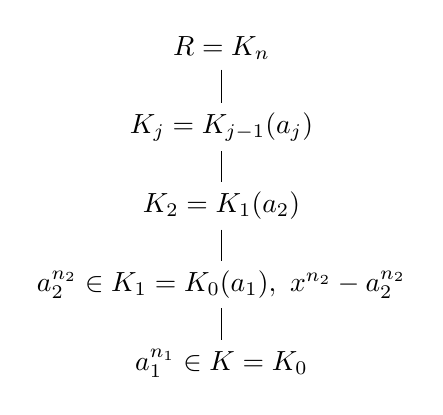
\begin{tikzpicture}[node distance=1cm and 2cm, auto]
            \node (R)  {$R = K_n$};
            \node (Kj) [below of =R] {$K_j = K_{j-1}(a_j)$};
            \node (K2) [below of =Kj] {$K_2 = K_1(a_2)$};
            \node (K1) [below of =K2] {$a_2^{n_2} \in K_1 = K_0(a_1),\ x^{n_2}-a_2^{n_2}$};
            \node (K0) [below of =K1] {$a_1^{n_1} \in K = K_0 $};
            \draw[-] (R) to node {}(Kj);
            \draw[-] (Kj) to node {}(K2);
            \draw[-] (K2) to node {}(K1);
            \draw[-] (K1) to node {}(K0);
        \end{tikzpicture}\\
    \end{center}
\end{dfn}

\begin{eg}[Ejemplos de radicales]
    \begin{enumerate}[a)]
        \item Ejemplo 1:\\$$\Q(e^{\frac{2\pi i}{n}})/\Q,\ \ \ \ (e^{\frac{2\pi i}{n}})^n = 1 \in \Q$$
        \item Ejemplo 2:\\

        \begin{center}
            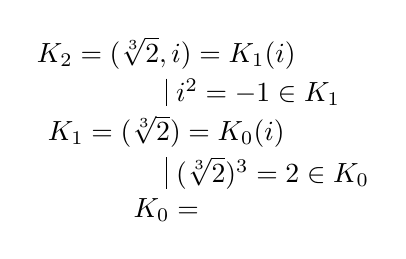
\begin{tikzpicture}[node distance=1cm and 2cm, auto]
                \node (A) {$ K_2 = \Q(\sqrt[3]{2}, i) = K_1(i) $};
                \node (B) [below of =A]{$ K_1 = \Q(\sqrt[3]{2}) = K_0(i)$};
                \node (C) [below of =B] {$ K_0 = \Q $};
                \draw[-] (A) to node {$i^2 = -1 \in K_1$}(B);
                \draw[-] (B) to node {$(\sqrt[3]{2})^3 = 2 \in K_0$}(C);
            \end{tikzpicture}\\
        \end{center}
        \item Ejemplo 3:\\

        \begin{center}
            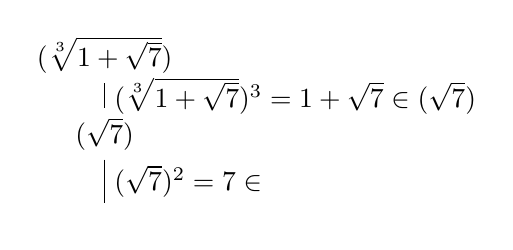
\begin{tikzpicture}[node distance=1cm and 2cm, auto]
                \node (A) {$ \Q(\sqrt[3]{1+\sqrt 7})$};
                \node (B) [below of =A]{$ \Q(\sqrt 7)$};
                \node (C) [below of =B] {$ \Q $};
                \draw[-] (A) to node {$(\sqrt[3]{1+\sqrt 7})^3 = 1 + \sqrt{7} \in \Q(\sqrt 7)$}(B);
                \draw[-] (B) to node {$(\sqrt 7)^2 = 7 \in \Q $}(C);
            \end{tikzpicture}\\
        \end{center}
    \end{enumerate}
\end{eg}

\begin{dfn}[Resolubilidad por radicales]
    $f \in K[x]$ es \textbf{resoluble por radicales} si existe alguna extensión radical $R/K$ tal que $K(f) \subseteq R$.
\end{dfn}

\begin{eg}[Ejemplos de resolubilidad por radicales]
    \begin{enumerate}[a)]
        \item $x^p-1$. $\Q(x^p-1) = \Q(e^{\frac{2\pi i}{p}})$.
        \item $x^4-2$. $\Q(\sqrt[4]{2}, i)$.
        \item $x^4+4x^2+2$. $\Q(\sqrt{2+\sqrt{2}})$.
    \end{enumerate}
\end{eg}

\section{Grupos resolubles}
Como se anticipó en la sección anterior, el \textit{Gran Teorema de Galois} utiliza el concepto de grupo resoluble, para ello vamos a definir los conceptos necesarios.

\begin{dfn}[Grupo simple]
    Sea $G$ un grupo, es \textbf{simple} si no tiene subgrupos normales.
\end{dfn}

\begin{obs}$ $
    \begin{itemize}
        \item $G$ abeliano es simple si $G \isom C_p$.
        \item Sea $G_m$ el subgrupo máximo normal de $G$. Entonces $G_m \normsub G$ y no hay normales entre $G_m$ y $G \implies \quo{G}{G_m}$ es simple.
    \end{itemize}
\end{obs}

\begin{obs}[Clasificación de grupos simples]
    Si $G$ es finito y simple, entonces:
    \begin{itemize}
        \item $G \isom C_p$, si son abelianos.
        \item $G \isom A_n: n\geq5$.
        \item $G$ es de tipo \textit{Lie}.
        \item 26 esporádicos.
    \end{itemize}
\end{obs}

Los grupos finitos simples tienen relevancia en teoría de grupos ya que informalmente son los \textit{bloques} que forman el resto de grupos finitos. En cierta forma un grupo simple es a un grupo finito lo que un número primo a un número natural. De la misma forma que se puede descomponer en factores primos a un número natural, podemos escribir una descomposición de un grupo en subgrupos simples.

\begin{dfn}[Serie de descomposición]
    Sea $G$ un grupo finito, y $\sdf{H_j}_{j=1}^{j=n}$ una sucesión de subgrupos tales que:
    $$
        \1 = H_0 \normsub H_1 \normsub \cdots \normsub H_n = G
    $$
    se llama a dicha cadena \textbf{serie de descomposición} del grupo si $\forall j,\ \quo{H_{j+1}}{H_j}$ es un grupo simple y $n$ es la longitud de la serie.
\end{dfn}

\begin{obs}
    Aunque queda fuera del temario, todas las series de descomposición de un mismo grupo $G$ son equivalentes salvo por permutaciones e isomorfismos.
\end{obs}

\begin{dfn}[Grupo resoluble]
    Un grupo $G$ es \textbf{resoluble} si existe una serie de descomposición de la forma:
    $$
        \sdf{e} = G_0 \normsubeq G_1 \normsubeq G_2 \normsubeq \cdots \normsubeq G_{n-1} \normsubeq G_n = G
    $$
    tal que $\quo{G_j}{G_{j-1}}$ es abeliano.
\end{dfn}

\begin{pro}[Resolubilidad de grupos abelianos]
    Todo grupo $G$ abeliano es resoluble, es decir:
    $$
        G \text{ abeliano} \implies G \text{ resoluble.}
    $$
\end{pro}
\begin{proof}
    Como $\sdf{1} \subseteq G$, y $\sdf{1} \normsub G$ dado que $x \cdot 1 \cdot x^{-1} \in \sdf{1}$ y además $\quo{G}{\sdf{1}} \isom G$ es abeliano, hemos encontrado una serie:
    $$
        \sdf{1 = e} \normsub G
    $$
    tal que $\quo{G_j}{G_{j-1}}$ es abeliano.
\end{proof}
\begin{eg}$ $
    \begin{enumerate}[i)]
        \item $A_4$ es resoluble. Sea $V = \gen{(12)(34), (13)(24)}$:\\

        \begin{center}
            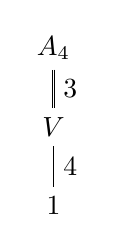
\begin{tikzpicture}[node distance=1cm and 2cm, auto]
                \node (A) {$ A_4 $};
                \node (B) [below of =A]{$ V $};
                \node (C) [below of =B] {$ \sdf{1} $};
                \draw[-, double] (A) to node {$3$}(B);
                \draw[-] (B) to node {$4$}(C);
            \end{tikzpicture}\\
        \end{center}
        \item $D_{2n}$ es resoluble.
        \item $S_3$ y $S_4$ son resolubles.
    \end{enumerate}
\end{eg}

\begin{obs}[Recuerdo de teoría de grupos]
    Sea $G$ un grupo, $N\normsubeq G$ y $H \leq G$ subgrupos y sea $M = H \cap N$, entonces:
    $$
        M \normsub H \text{ y } \quo{H}{M} \isom \quo{HN}{N}
    $$
    \begin{center}
        \begin{tikzpicture}[node distance=1cm and 2cm, auto]
            \node (A) {$N$};
            \node (B) [right= of A] {$ $};
            \node (C) [right= of B] {$H$};
            \node (D) [above of =B] {$G$};
            \node (E) [below of =B] {$N\cap H = M$};
            \node (F) [below of =E] {$\1$};
            \draw[-, double] (D) to node {}(A);
            \draw[-] (D) to node {}(C);
            \draw[-] (A) to node {}(E);
            \draw[-] (C) to node {}(E);
            \draw[-] (E) to node {}(F);
        \end{tikzpicture}\\
    \end{center}
\end{obs}

\section{Resolubilidad y extensiones de Galois}

En esta sección vamos a ver resultados que relacionen los conceptos de un radical $R/K$ con extensiones de Galois, ya que en general un radical no es una extensión de Galois, como por ejemplo $\Q(\sqrt[4]{2})/\Q$ y
$\Q(\sqrt{1+\sqrt 7})/\Q$.

\begin{thm}[Kummer]\label{thm:5.1}
    Sean $E, K$ cuerpos de la forma $\Q \subseteq K \subseteq E \subseteq \C$, si $K$ contiene $\xi \in \C$ con $o(\xi) = n$, entonces son equivalentes:
    \begin{enumerate}[a)]
        \item $E = K(a)$ con $a \in E$ tal que $a^n \in K$.
        \item $E/K$ es una extensión de Galois con $\gal(E/K)$ cíclico de orden un divisor de $n$.
    \end{enumerate}
\end{thm}

\begin{proof}$ $
    \begin{enumerate}
        \item[a) $\implies$ b)] Tenemos que $E = K(a)$ con $a^n \in K$. Podemos suponer que $a \notin \K$. Sea $f(x) = x^n - a^n \in K[x]$, las raíces de $f$ son $\sdf{a\xi^j \mid 0 \leq j \leq n}$.
        Como $E = K(a) = K(a\xi^j\mid 0 \leq j \leq n) = K(x^n - a^n)$, entonces $E/K$ es de Galois.\\
        Sea $\sigma \in \gal(E/K)$, $\sigma(a) = a\xi^{\kappa_\sigma}$ donde $0 \leq \kappa_\sigma \leq n$. Definimos:\\
        \begin{center}
            \begin{tikzpicture}[node distance=1cm and 2cm, auto]
                \node (B)                {$\sigma$};
                \node (A)  [above of =B] {$\rho: \gal(E/K)$};
                \node (E)  [right= of B] {$\xi^{\kappa_\sigma}$};
                \node (D)  [above of =E] {$\gen{\xi}$};
                \draw[->]  (A) to node {}(D);
                \draw[|->] (B) to node {}(E);
            \end{tikzpicture}\\
        \end{center}
        Y entonces:
        \begin{itemize}
            \item $\rho(\1_E) = \rho^0 = 1$
            \item $\rho(\sigma\tau) = \xi^{\kappa_\sigma+\kappa_\tau} \xi^{\kappa_\sigma} * \xi^{\kappa_\tau} = \rho(\sigma)\rho(\tau)$.
            Donde $\sigma\tau(a) = \tau(a \xi^{\kappa_\sigma}) = a \xi^{\kappa_\tau} \xi^{\kappa_\sigma} = \xi^{\kappa_\sigma+\kappa_\tau}$
            \item $\rho$ es inyectiva porque $\rho(\sigma) = 1 \implies \sigma(a) = a \implies \sigma = 1_E$ y por tanto $\gal(E/K) \leq \gen{\xi}$.
        \end{itemize}
        \item[b) $\implies$ a)] Como $E/K$ es de Galois, $\gal(E/K) = \gen{\tau}$ y sea $n$ el orden del grupo de Galois, entonces: $o(\tau) = d\divides n$ y $\vabs{E:K} = d$.

        Sea $\omega \in\gen{\xi}$ tal que $o(\omega) = d$ (por ejemplo $\omega = \xi^{\frac{n}{d}})$, basta encontrar un $a \in E$ tal que $\tau(a) = a\omega$ y $a \notin K$. Vamos a ver por qué:\\
        Supongamos que existe tal $a$, entonces:
        $$
            \tau(a^d) = (\tau(a))^d = a^d \omega^d = a^d \implies a^d \in E^\gen{\tau} = K.
        $$
        En particular, $a^n = (a^d)^{\frac{n}{d}} \in K$. Sea $p = Irr(K, a) \in K[x]$, $p \divides x^d - a^d$.
        Por otro lado, $a, a\omega = \tau(a), \ldots, a\omega^{d-1} = \tau^{d-1}(a)$ son raíces de $p$ distintas $\implies \delta(p) \geq d \implies p(x) = x^d - a^d$, por tanto:
        $$
            \vabs{K(a):K} = \delta(p) = d = \vabs{E:K} \implies E = K(a)
        $$

        Finalmente, solo nos queda buscar el $a$ que mencionamos arriba. Por el \hyperref[thm:4.2]{teorema de Dedekind}, $\sdf{1, \tau, \ldots, \tau^{d-1}}$ es linealmente independiente y entonces:
        $$
            \1 + \frac{1}{\omega} \tau + \cdots + \frac{1}{\omega^{d-1}}\tau^{d-1} \neq 0
        $$
        Sea $b \in E$ tal que $0 \neq b + \frac{1}{\omega} \tau(b) + \cdots + \frac{1}{\omega^{d-1}}\tau^{d-1}(b) = a$ y hemos encontrado el $a$ que buscábamos. Puede comprobarse que $\tau(a) = \omega a = a \omega$.
    \end{enumerate}
\end{proof}

El siguiente grafo resume el resultado del teorema:\\
\begin{center}
    \begin{tikzpicture}[edge quotes mid, node distance=1cm and 2cm, auto]
        \node (A) [above of =C]{$E(\xi) = \gen{K(\xi), E}$};
        \node (B) [] {$K(\xi)$};
        \node (C) [right= of B] {$ $};
        \node (D) [right= of C] {$E = K(a)$};
        \node (E) [below of =C] {$K(\xi)\cap E$};
        \node (F) [below of =E] {$K$};
        \draw[-] (A) to node [sloped]{abeliana}(B);
        \draw[-] (A) to node {}(D);
        \draw[-] (B) to node {}(E);
        \draw[-] (D) to node {}(E);
        \draw[-] (B) to node [sloped, below]{abeliana}(F);
    \end{tikzpicture}\\
\end{center}

\begin{ex}[H5.2]
    Sea $E/K$ una extensión de Galois, $K \subseteq L, M \subseteq E$ subcuerpos intermedios. $\gen{L, M} = \bigcap_{H \subseteq E} H$ tal que   $L,M \subseteq H$. Prueba que:
    $$
        \gal(E/L) \cap \gal(E/M) = \gal(E/\gen{L, M})
    $$
    \textbf{Solución}\\\\

    Vamos a resolverlo por doble inclusión. Por definición $\gal(E/\gen{L, M}) \subseteq \gal(E/L) \cap \gal(E/M)$.\\
    Además $L,M\subseteq E^{\gal(E/L) \cap \gal(E/M)} \subseteq E$ y $\gen{L, M} \subseteq E^{\gal(E/L) \cap \gal(E/M)}$. Por tanto:
    $$
        \gal(E/E^{\gal(E/L) \cap \gal(E/M)}) \subseteq \gal(E/\gen{L, M})
    $$
    y $\gal(E/L) \cap \gal(E/M) = \gal(E/E^{\gal(E/L) \cap \gal(E/M)})$ por el \hyperref[thm:fund-gal]{TFTG}.
\end{ex}

\begin{ex}[H5.4]
    Por completar. %TODO
\end{ex}

\section{Gran Teorema de Galois}

\textit{NOTA: Solo están redactados los resultados teóricos de esta sección. Todos los ejercicios de esta sección están por redactar (se corresponden con H5.8, H5.10, H5.11, H5.12, H5.5, H5.6). También falta algún ejemplo, y las pruebas de los resultados.}

\begin{obs}[Recuerdo de teoría de grupos]
    Sea $G$ un grupo y $N \normsubeq G$, $H \leq G$ subgrupos, entonces:
    \begin{enumerate}[a)]
        \item $NH \leq G$, $N \cap H \normsubeq H$ y además $$\quo{NH}{N} \isom \quo{H}{N\cap H}$$.
        \item Si además $H \normsub G$, entonces $NH \normsub G$, $H  \normsubeq NH$ y además:
        $$
            \quo{G}{NH} \isom \quo{\quo{G}{N}}{\quo{NH}{N}}
        $$
    \end{enumerate}
\end{obs}

\begin{dfn}[Extensión abeliana]
    Una extensión $E/K$ es \textbf{abeliana} si $E/K$ es de Galois y $\gal(E/K)$ es un grupo abeliano.
\end{dfn}

\begin{lm}[Extensión de Galois y resoluble]\label{lm:5.2}
    Sea $\Q \subseteq K$, $L \subseteq \C$ y $L/K$ una extensión. Supongamos que existe una sucesión $\sdf{K_j}_{j=0}^{j=m}$ tal que $K = K_0$, $L = K_m$ monótona creciente por inclusión y $K_j/K_{j-1}$ es abeliana. Entonces si $E/K$ es de Galois, con $E \subseteq L$, entonces $\gal(E/K)$ es resoluble.
\end{lm}
\begin{proof}
    A completar.
\end{proof}
\begin{thm}[Gran Teorema de Galois]\label{thm:5.3}\label{thm:GTG}
    Sea $\Q \subseteq K$ un cuerpo, $f \in K[x]$ un polinomio y $E = K(f) \subseteq \C$ su cuerpo de escisión.
    $$
        f \text{ es resoluble por radicales } \iff \gal(f) = \gal(E/K) \text{ es resoluble }
    $$
\end{thm}
\begin{proof}
    A completar.
\end{proof}

\begin{lm}[Generación del grupo simétrico]\label{lm:5.4}
    Para $n \leq 2$, $S_n = \gen{(12)(12\cdots n)}$
\end{lm}

\begin{thm}[de Abel-Ruffini]
    Las ecuaciones polinómicas \textbf{generales} $f(x) = a_n x^n + \cdots + a_1 x + a_0 = 0$ no son resolubles por radicales cuando $\delta(f)\geq 5$. Es decir, no es posible encontrar las soluciones de $f$ de forma general aplicando finitamente la suma, resta, multiplicación y radicación.
\end{thm}

\begin{proof}
    A completar.
\end{proof}

\begin{obs}
    Equivalentemente, el teorema enuncia que no existe una fórmula general para hallar las raíces de $f(x)$ con $\delta(f) \geq 5$ aplicada a sus coeficientes. Para $\delta(f) \leq 4$ si es posible, por ejemplo con $\delta(f) = 2$ tenemos:
    $$
        x = \frac{-b \pm \sqrt{b^2-4ac}}{2a}
    $$
    Existen también fórmulas para polinomios de tercer y cuarto grado.
\end{obs}
